\pagebreak

\subsection{Архитектура на софтуерната програма}
Софтуерната програма е съставена от 4 модула, които комуникират помежду си.

\begin{figure}[here]
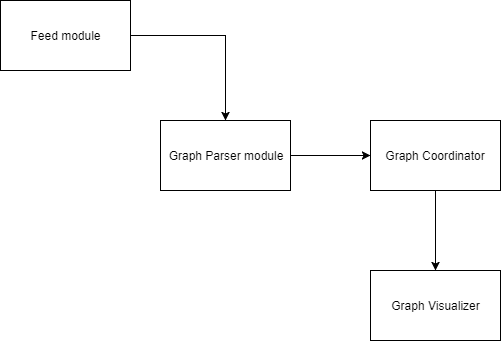
\includegraphics{modules}
\caption{Архитектура на софтуерната програма}
\label{fig:architecture}
\end{figure}

\begin{itemize}
    \item Feed  модул, който има за отговорност да захранва с данни останалите модули с граф, който за всяка точка съдържа разстояниято между точката и всички останали точки. Ако разстоянието между две точки не може да бъде измерено то тогава разстоянието се означава с специален флаг поле, което е дефинирано като -безкрайност.
    \item Graph Parser модул, който има за цел да обработи информацията, която ‘Feed’ модулът изпраща и да я трансформира в друг граф – който държи информацията във върхове и дъги. Върховете и 
    дъгите съдържат информация, която помага за визуализацията на графа в 3D.
    \item Graph Coordinator модул, който има за цел да определи -координатите в пространството на всички обекти, които се съдържат в графа, който се получава в резултат на стъпка 2 (Graph Parser). Координатите се определят чрез система от линейни уравнения, които считат, че началната позиция на стационарните обекти е (0,0,0) - в един от ъглите на мястото, в което щже бъдат следени обектите.
    \item Graph Visualizer модул, който има за цел да използва графа, чиито координати са били вече определени от Graph Coordinator и да ги визуализира по удачен начин в 3 измерения.
\end{itemize}